\documentclass[11pt,letterpaper]{article}
\usepackage[T1]{fontenc}
\usepackage{mathpazo}
\renewcommand{\ttdefault}{pcr}
\usepackage[margin=1in,headheight=15pt]{geometry}
\usepackage{amsmath,amssymb,amsthm,mathtools}
\usepackage{microtype,graphicx,booktabs,array,enumitem,placeins}
\usepackage{xcolor,fancyhdr}
\definecolor{ink}{HTML}{18354A}
\definecolor{teal}{HTML}{167D8D}
\usepackage[colorlinks=true,linkcolor=ink,citecolor=teal,urlcolor=teal,hypertexnames=false]{hyperref}
\hypersetup{pdftitle={Flattening a Sphere Almost Everywhere: Verification and Explanation},pdfauthor={Mathematical verification prepared for Vladimir Reshetnikov}}
\pagestyle{fancy}
\fancyhf{}
\fancyhead[L]{\small\textsc{Flattening a sphere almost everywhere}}
\fancyhead[R]{\small Verification and explanation}
\fancyfoot[C]{\thepage}
\setlength{\parindent}{0pt}
\setlength{\parskip}{0.48em}
\setlist{topsep=0.3em,itemsep=0.2em,parsep=0pt}
\setlength{\emergencystretch}{2em}
\numberwithin{equation}{section}
\setcounter{tocdepth}{1}
\newtheorem{theorem}{Theorem}[section]
\newtheorem{proposition}[theorem]{Proposition}
\newtheorem{lemma}[theorem]{Lemma}
\newtheorem{corollary}[theorem]{Corollary}
\theoremstyle{remark}
\newtheorem{remark}[theorem]{Remark}
\newcommand{\R}{\mathbb R}
\newcommand{\dd}{\,\mathrm d}
\newcommand{\area}{\operatorname{area}}
\newcommand{\dist}{\operatorname{dist}}
\newcommand{\diam}{\operatorname{diam}}
\newcommand{\Lip}{\operatorname{Lip}}
\newcommand{\eps}{\varepsilon}
\newcommand{\norm}[1]{\left\lVert#1\right\rVert}
\newcommand{\abs}[1]{\left\lvert#1\right\rvert}
\newcommand{\closure}[1]{\overline{#1}}
\newcommand{\m}{\mathcal L}
\newcommand{\Good}{E}
\newcommand{\Bad}{Z}

\begin{document}
\begin{center}
{\color{teal}\small MATHEMATICAL VERIFICATION}\par\vspace{0.6em}
{\color{ink}\LARGE\bfseries Flattening a Sphere\par Almost Everywhere}\par\vspace{0.65em}
{\large A complete proof, its precise meaning,\par and the limits of the claim}\par\vspace{0.8em}
Prepared for Vladimir Reshetnikov\par
23 November 2026
\end{center}

\begin{abstract}
The main existence claim in the supplied document is correct. A sphere with a closed meridian removed admits a homeomorphism to a planar domain whose classical differential is an isometry at almost every spherical point. The map can be uniformly close to the sinusoidal projection, with arbitrarily small positive excess area. The refinement estimates in the document do prove classical, not merely approximate, differentiability. This report supplies a complete proof, simplifies the construction to one mesh size per stage, repairs a minor parameter-range issue, and expands the measure-theoretic steps. It also establishes sharper consequences: the map is not locally Lipschitz on any open patch; the exceptional image has positive area in every planar open set; and the particular construction has explicit positive excess area. The result preserves first-order geometry almost everywhere, but does not preserve all finite distances, curve lengths, or areas. A separate application of an existing theorem gives zero excess area under approximate differentiability; the corresponding classical question is not settled here. No claim of historical novelty is certified.
\end{abstract}

\tableofcontents
\newpage

\section{Verdict and the precise theorem}
\label{sec:verdict}

The supplied note~\cite{source} contains a valid construction. Its most important estimate is the local perturbation bound inside an old affine tile. That estimate, together with a rapidly shrinking mesh, controls the difference quotient along \emph{every} approach to almost every base point. Merely showing convergence of derivatives on sets of large measure would not suffice; the note does more than that.

The phrase ``no distortion at almost every point'' must be read in its stated differential sense. It does not mean that a physical sheet can be flattened without stretching, that every path retains its length, or that every measurable region retains its area.

Let
\[
 D=(-\pi,\pi)\times(-\pi/2,\pi/2),\qquad
 \Phi(x,y)=(\cos y\cos x,\cos y\sin x,\sin y).
\]
The image $S=\Phi(D)$ is the unit sphere with the meridian at longitude $\pi$, including both poles, removed. The missing meridian has spherical area zero, so $\area(S)=4\pi$. The map $\Phi$ is a smooth coordinate parametrization of $S$.

\begin{theorem}[Verified flattening theorem]
\label{thm:main}
For every $\eps>0$ there are a bounded open set $\Omega\subset\R^2$, a homeomorphism $F:S\to\Omega$, and a Borel set $Z\subset S$ of spherical area zero such that:
\begin{enumerate}[label=(\roman*)]
\item $4\pi<\area(\Omega)<4\pi(1+\eps)$.
\item At every $p\in S\setminus Z$, $F$ is classically differentiable and its differential $dF_p:T_pS\to\R^2$ is a linear isometry.
\item $\area(F(S\setminus Z))=4\pi$. At every point of this image, $F^{-1}$ is classically differentiable, with isometric differential.
\item If $P(\Phi(x,y))=(x\cos y,y)$ is the sinusoidal projection, then
\[
 \sup_{p\in S}|F(p)-P(p)|<2\eps.
\]
\end{enumerate}
Moreover, this $F$ is not locally Lipschitz on any nonempty open patch. The set $F(Z)$ has positive area in every nonempty open subset of $\Omega$.
\end{theorem}

The lower bound in (i), and the last statement about every open subset, strengthen the supplied formulation. They describe this construction; the theorem is not a general impossibility result for all exact-area maps.

\subsection{Corrections and qualifications to the supplied note}

\begin{enumerate}
\item \textbf{Parameter range.} The scalar proposition assumes its parameter is less than $1$. To prove the final theorem for arbitrary $\eps>0$, use
\begin{equation}\label{eq:delta}
 \delta=\min\{\eps/3,1/2\}
\end{equation}
in that proposition. The unconditional substitution $\eps/3$ needs this small adjustment.
\item \textbf{Almost every parallel.} Two-dimensional almost-everywhere differentiability implies the claimed one-dimensional derivative on \emph{almost every} latitude, not automatically on every latitude. Fubini's theorem provides exactly what the area calculation needs.
\item \textbf{The inverse's good set.} The inverse is isometric to first order on a set of planar area $4\pi$. This is \emph{not} a full-measure subset of $\Omega$, because $\area(\Omega)>4\pi$.
\item \textbf{The ``sliver.''} The exceptional image has small total area, but it is not confined to a thin border. It has positive area in every open portion of the sheet.
\item \textbf{Lipschitz terminology.} The local statement is unambiguous. A global Lipschitz comparison for a cut sphere must specify its metric: the intrinsic path metric of the cut surface and the distance inherited from the uncut sphere behave differently across the seam.
\item \textbf{Exact area and novelty.} ``Zero excess area'' is a separate question. It cannot mean substituting $\eps=0$ literally into all four clauses. The literature check below verifies neighboring results, but does not certify priority or settle the classical exact-area question.
\end{enumerate}

\section{How almost-everywhere rigidity can coexist with distortion}
\label{sec:meaning}

\subsection{The one-dimensional model}

Let $C:[0,1]\to[0,1]$ be the Cantor staircase. It is continuous, nondecreasing, has $C(0)=0$, $C(1)=1$, and has derivative zero almost everywhere. For $\alpha>0$, define
\[
 f(t)=t+\alpha C(t).
\]
Then $f$ is a strictly increasing homeomorphism from $[0,1]$ onto $[0,1+\alpha]$ and
\[
 f'(t)=1\quad\text{for almost every }t,
 \qquad f(1)-f(0)=1+\alpha.
\]
Thus unit derivative almost everywhere does not force preservation of the length of the whole interval. The missing hypothesis is absolute continuity. The Cantor staircase contributes a singular increase that is invisible to its almost-everywhere classical derivative.

If $K$ is the usual zero-length Cantor set, the intervals making up $[0,1]\setminus K$ retain their lengths under $f$, because $C$ is constant on each of them. Their images have total length $1$. Consequently,
\[
 |f(K)|=\alpha.
\]
A null set has acquired positive measure under a continuous one-to-one map. This is the basic mechanism behind the spherical construction.

\begin{figure}[htbp]
\centering
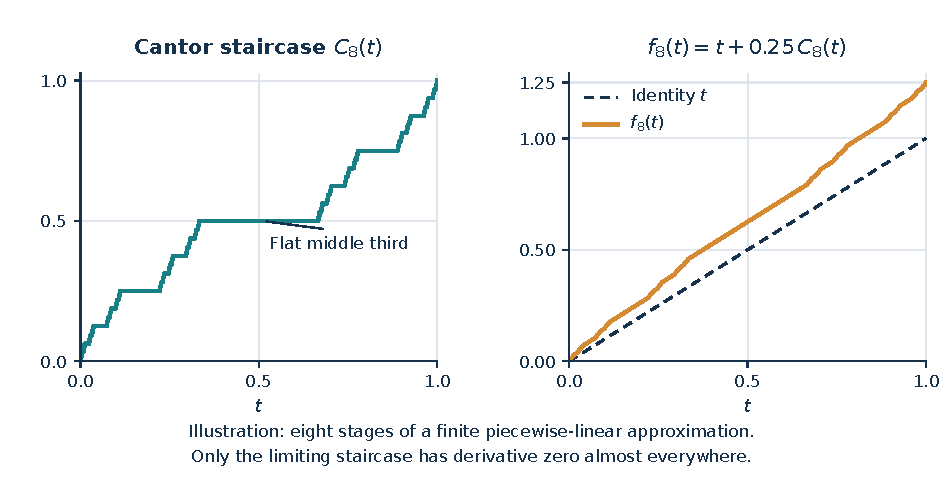
\includegraphics[width=\textwidth]{figures/singular_staircase.pdf}
\caption{A finite polygonal approximation illustrates the Cantor staircase mechanism. The almost-everywhere derivative statements concern the limiting functions, not these finite approximants.}
\label{fig:cantor}
\end{figure}

\subsection{What is harder in two dimensions}

The spherical metric in the coordinates above is
\begin{equation}\label{eq:metric}
 ds^2=\cos^2 y\,dx^2+dy^2,
 \qquad dA=\cos y\,dx\,dy.
\end{equation}
We seek a triangular map
\[
 G(x,y)=(u(x,y),y),\qquad F=G\circ\Phi^{-1},
\]
with
\begin{equation}\label{eq:desired}
 \nabla u(x,y)=(\cos y,0)\quad\text{almost everywhere}.
\end{equation}
At such points,
\[
 DG=\begin{pmatrix}\cos y&0\\0&1\end{pmatrix},
 \qquad DG^{\mathsf T}DG=\begin{pmatrix}\cos^2y&0\\0&1\end{pmatrix}.
\]
The equality of these quadratic forms is exactly preservation of tangent-vector lengths and angles.

The sinusoidal projection has coordinate derivative
\[
 D(x\cos y,y)=\begin{pmatrix}\cos y&-x\sin y\\0&1\end{pmatrix}.
\]
Its nonzero upper-right entry is a shear. A naive formula $x\cos y+\alpha C(x)$ does not remove that shear: its latitude derivative is still $-x\sin y$.

The construction must coordinate singular staircases across latitudes. It repeatedly makes $u$ independent of latitude on most small rectangles, then joins the pieces across very thin layers. These layers and the horizontal catch-up intervals occupy a summable fraction of area. Their gradients can be large; their function values move only a little.

\subsection{Why curvature is not contradicted}

A smooth local isometry from a spherical patch to the plane is impossible because Gaussian curvature is preserved under local isometry, while the two curvatures are $1$ and $0$. The obstruction persists for locally Lipschitz homeomorphisms with isometric differential almost everywhere; a precise regularity theorem is discussed in Section~\ref{sec:regularity}.

The constructed map lies outside that regularity class on every open patch. Its classical derivative exists almost everywhere, but integrating those derivatives does not recover all of its increments. In particular, one cannot infer curve-length preservation by integrating its almost-everywhere speed.

\FloatBarrier
\section{The scalar proposition}
\label{sec:scalar}

\begin{proposition}[Monotone prescribed gradient]
\label{prop:scalar}
For every $0<\delta<1$ there is $u\in C(\closure D)$ satisfying:
\begin{align}
 u(x_2,y)-u(x_1,y)&\ge\cos y\,(x_2-x_1)
 &&(x_1<x_2),\label{eq:mono}\\
 |u(x,y)-(\cos y+\delta)x|&\le\delta
 &&((x,y)\in\closure D),\label{eq:close}\\
 Du(x,y)&=(\cos y,0)
 &&\text{for almost every }(x,y)\in D.\label{eq:gradient}
\end{align}
Here $Du$ is the classical two-variable derivative.
\end{proposition}

We prove the proposition in detail. Unlike the supplied proof, we take equal longitude and latitude mesh sizes. This removes a parameter without changing any of the essential estimates.

For $n\ge0$, set
\[
 \gamma_n(y)=\cos y+\delta4^{-n}.
\]
For $n\ge1$, set $\theta_n=2^{-n-3}$. Start with
\[
 u_0(x,y)=\gamma_0(y)x,\qquad\rho_0=\delta.
\]
The induction maintains the lower-slope condition
\begin{equation}\label{eq:H}
 u_n(x_2,y)-u_n(x_1,y)\ge\gamma_n(y)(x_2-x_1).
 \tag{$H_n$}
\end{equation}

\subsection{Selecting the mesh}

Suppose $u_{n-1}$ is constructed. Let
\[
 \omega_{n-1}(t)=\sup\bigl\{
 |u_{n-1}(z)-u_{n-1}(w)|:
 z,w\in\closure D,\ |z-w|\le t\bigr\}.
\]
Continuity on the compact rectangle gives $\omega_{n-1}(t)\to0$ as $t\to0$. Choose an integer $N_n$ large enough that $h_n=\pi/N_n$ satisfies
\begin{align}
 h_n&\le3\delta4^{-n},\label{eq:scale1}\\
 2h_n&\le\rho_{n-1}/2,\label{eq:scale2}\\
 2\omega_{n-1}(h_n)&\le2^{-n}\rho_{n-1}.\label{eq:scale3}
\end{align}
Put
\[
 M_n=2N_n,\qquad \rho_n=\theta_nh_n.
\]
All three requirements can be met by increasing $N_n$. In particular $\rho_n\to0$ and $\rho_n<\rho_{n-1}$.

\subsection{One refinement}

For this subsection write $h=h_n$, $\theta=\theta_n$, $N=N_n$, $M=M_n$. Define
\[
 y_j=-\pi/2+jh,\quad J_j=[y_j,y_{j+1}],\quad
 \bar y_j=(y_j+y_{j+1})/2
\]
for $0\le j<N$, and $x_k=-\pi+kh$ for $0\le k\le M$. The enlarged strip is
\[
 J_j^+=\{y\in[-\pi/2,\pi/2]:\dist(y,J_j)\le\theta h\}.
\]
Set
\[
 b_j=\max_{y\in J_j^+}\gamma_n(y),\qquad
 P_j(x)=u_{n-1}(x,\bar y_j).
\]
On each interval $[x_k,x_{k+1}]$, define $Q_j$ by
\begin{equation}\label{eq:Q}
 Q_j(x_k+t)=P_j(x_k)+b_jt
 \quad(0\le t\le(1-\theta)h),
\end{equation}
and then join linearly to $Q_j(x_{k+1})=P_j(x_{k+1})$ on the remaining interval of length $\theta h$.

Away from the interior latitude grid lines by at least $\theta h$, set $u_n(x,y)=Q_j(x)$ in strip $J_j$. Within the layer $|y-y_j|\le\theta h$ at an interior grid line, set
\begin{equation}\label{eq:layer}
 u_n(x,y)=(1-t)Q_{j-1}(x)+tQ_j(x),\qquad
 t=\frac{y-y_j+\theta h}{2\theta h}.
\end{equation}
These definitions agree on their boundaries. Since $\theta\le1/16$, distinct latitude interpolation layers do not overlap.

The \emph{tiles} are the open rectangles where $x$ lies in the long first part of a longitude interval and $y$ lies in the open core of a latitude strip. On each such tile,
\begin{equation}\label{eq:tile}
 u_n(x,y)=a+b_jx.
\end{equation}

\begin{figure}[htbp]
\centering
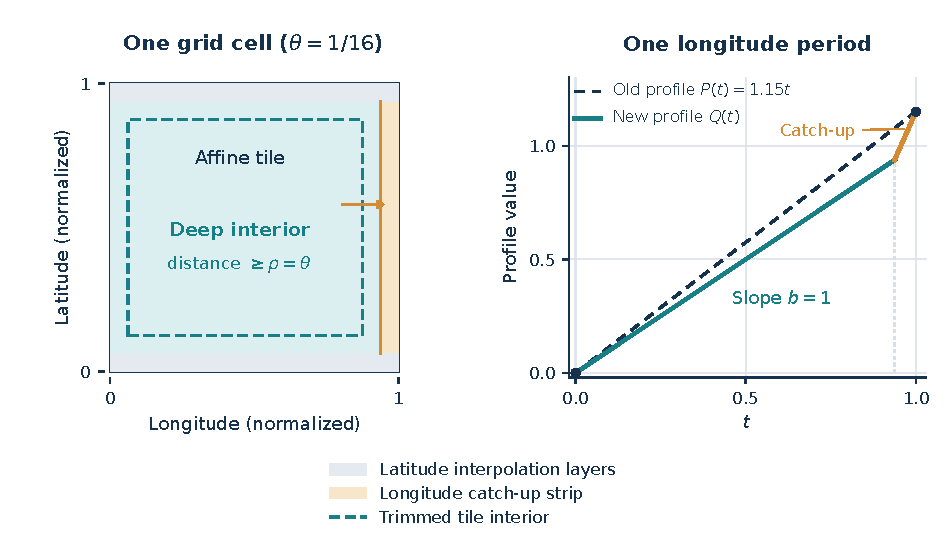
\includegraphics[width=\textwidth]{figures/refinement_stage.pdf}
\caption{A normalized refinement cell and an illustrative re-profiled affine function. The long interval has the desired smaller slope; the short catch-up interval restores the old endpoint value. Latitude interpolation occurs only in thin horizontal layers. The actual proof uses successively much smaller meshes.}
\label{fig:refinement}
\end{figure}

\subsection{Five estimates, with proofs}

\paragraph{1. Preservation of the lower slope.}
Every point of $J_j^+$ is within $(1/2+\theta)h<h$ of $\bar y_j$. Since $\gamma_n$ is $1$-Lipschitz,
\begin{equation}\label{eq:bjbound}
 b_j\le\gamma_n(\bar y_j)+h
 \le\gamma_n(\bar y_j)+3\delta4^{-n}
 =\gamma_{n-1}(\bar y_j).
\end{equation}
By $(H_{n-1})$, the endpoint rise of $P_j$ on a period is at least $b_jh$. After using $b_j(1-\theta)h$ on its long part, the remaining rise is at least $b_j\theta h$. Thus the catch-up slope is at least $b_j$ as well.

In a core, $b_j\ge\gamma_n(y)$. In a latitude layer, $y$ lies in both enlarged neighboring strips, so both profiles in~\eqref{eq:layer} have lower slope at least $\gamma_n(y)$. Convex interpolation preserves this lower bound. This proves $(H_n)$ and continuity of $u_n$.

\paragraph{2. Accuracy of the affine tiles.}
On a tile, $Du_n=(b_j,0)$. For every $y\in J_j$,
\begin{equation}\label{eq:tileaccuracy}
 0<b_j-\cos y\le2h_n+\delta4^{-n}.
\end{equation}
Indeed, the $\delta4^{-n}$ term is positive, and the latitude arguments used in the maximum differ from $y$ by less than $2h_n$.

\paragraph{3. Uniform change at one stage.}
Both $P_j$ and $Q_j$ are increasing and share the endpoint values of each longitude interval. Therefore their difference anywhere in that interval is bounded by the oscillation of $P_j$ there, at most $\omega_{n-1}(h_n)$. Freezing the latitude at the relevant midpoint adds at most another $\omega_{n-1}(h_n)$; every midpoint used is within $h_n$ of the current latitude. The same bound holds after convex interpolation. Hence
\begin{equation}\label{eq:uniformstage}
 \norm{u_n-u_{n-1}}_\infty
 \le2\omega_{n-1}(h_n)
 \le2^{-n}\rho_{n-1}.
\end{equation}

\paragraph{4. Improved change inside an old tile.}
Suppose $n\ge2$, and $z$ belongs to a stage-$(n-1)$ tile $T'$ with distance at least $2h_n$ from its boundary. Write the old function there as $a+b'x$. All longitude endpoints and latitude midpoints used to compute $u_n(z)$ remain in that same tile: their distance from $z$ is at most $2h_n$. The relevant frozen old profiles are therefore the same affine function.

For each profile used at $z$, the slope estimates imply
\begin{align*}
 \gamma_{n-1}(\bar y_j)-3\delta4^{-n}
 &\le b_j\le\gamma_{n-1}(\bar y_j),\\
 \gamma_{n-1}(\bar y_j)
 &\le b'\le\gamma_{n-1}(\bar y_j)+2h_{n-1}.
\end{align*}
Consequently,
\begin{equation}\label{eq:eta}
 0\le b'-b_j\le\eta_n,
 \qquad\eta_n:=2h_{n-1}+3\delta4^{-n}.
\end{equation}
The difference $Q_j-P_j$ vanishes at both period endpoints, falls linearly on the long part, and returns linearly on the short part. Its magnitude is at most $(b'-b_j)h_n$. Convex interpolation does not increase this bound, so
\begin{equation}\label{eq:localstage}
 |u_n(z)-u_{n-1}(z)|\le\eta_nh_n.
\end{equation}
This is the key estimate. It is much better than the global bound at points lying safely inside old tiles.

\paragraph{5. Most points lie deep inside a tile.}
Let $K_n$ be the union of the closed stage-$n$ tiles trimmed inward by $\rho_n=\theta_nh_n$. Before trimming, a tile has width $(1-\theta_n)h_n$ and height at least $(1-2\theta_n)h_n$. After trimming, its dimensions are at least
\[
 (1-3\theta_n)h_n\quad\text{and}\quad(1-4\theta_n)h_n.
\]
Thus the retained fraction of each grid cell is at least
\[
 (1-3\theta_n)(1-4\theta_n)\ge1-7\theta_n,
\]
and
\begin{equation}\label{eq:badmeasure}
 |D\setminus K_n|\le7\theta_n|D|.
\end{equation}
The boundary rows have no larger loss. Grid boundaries themselves have zero area.

\subsection{Uniform convergence and monotonicity}

Because $\rho_{n-1}\le\rho_0=\delta$, equation~\eqref{eq:uniformstage} gives
\[
 \sum_{n\ge1}\norm{u_n-u_{n-1}}_\infty
 \le\sum_{n\ge1}2^{-n}\rho_{n-1}\le\delta.
\]
The sequence converges uniformly on $\closure D$ to a continuous function $u$, and~\eqref{eq:close} follows from the formula for $u_0$. Passing to the limit in $(H_n)$ gives~\eqref{eq:mono}.

\FloatBarrier
\section{Why the limit is classically differentiable almost everywhere}
\label{sec:diff}

Define the Borel set
\begin{equation}\label{eq:E}
 E=\bigcup_{N\ge1}\bigcap_{n\ge N}K_n.
\end{equation}
Since $\sum_n\theta_n<\infty$, equation~\eqref{eq:badmeasure} and the first Borel--Cantelli lemma give $|D\setminus E|=0$. Independence is not needed: the measure of points in infinitely many bad sets is bounded by each tail of the summable series.

Fix $p=(x_0,y_0)\in E$. There is $n_0$ such that for every $n\ge n_0$, $p$ lies in a stage-$n$ tile $T_n$ at distance at least $\rho_n$ from its boundary.

Let $q=(x,y)\ne p$ be any sufficiently nearby point of $D$, and put $r=|q-p|$. Choose $n\ge n_0$ such that
\begin{equation}\label{eq:choose-n}
 \rho_{n+1}/2\le r<\rho_n/2.
\end{equation}
Both $p$ and $q$ lie in $T_n$ with distance at least $\rho_n/2$ from its boundary. By~\eqref{eq:scale2}, this is at least $2h_{n+1}$. Write $u_n=a+\beta_nx$ on $T_n$. Then
\begin{align}
 u(q)-u(p)-\cos y_0(x-x_0)
 ={}&(\beta_n-\cos y_0)(x-x_0)\notag\\
 &+(u-u_n)(q)-(u-u_n)(p).\label{eq:diffsplit}
\end{align}
The first term is bounded in absolute value by
\[
 (2h_n+\delta4^{-n})r.
\]
For either $z=p$ or $z=q$, apply the improved local estimate to stage $n+1$ and the global estimate to all subsequent stages:
\begin{align}
 |(u-u_n)(z)|
 &\le\eta_{n+1}h_{n+1}
   +\sum_{m\ge n+2}2^{-m}\rho_{m-1}\notag\\
 &\le\eta_{n+1}h_{n+1}
   +2^{-n-1}\rho_{n+1}\notag\\
 &\le\left(\frac{2\eta_{n+1}}{\theta_{n+1}}+2^{-n}\right)r.
 \label{eq:tail}
\end{align}
The last line uses the lower bound on $r$ in~\eqref{eq:choose-n}. Finally,
\begin{align}
 \eta_{n+1}
 &=2h_n+3\delta4^{-(n+1)}
 \le\frac{27}{4}\delta4^{-n},\notag\\
 \frac{\eta_{n+1}}{\theta_{n+1}}
 &\le108\delta2^{-n}\longrightarrow0.\label{eq:108}
\end{align}
Combining~\eqref{eq:diffsplit}--\eqref{eq:108} yields the explicit difference-quotient estimate
\begin{equation}\label{eq:finaldiff}
 \frac{|u(q)-u(p)-\cos y_0(x-x_0)|}{|q-p|}
 \le2h_n+\delta4^{-n}+432\delta2^{-n}+2^{1-n}.
\end{equation}
The right-hand side tends to zero as $q\to p$, since then $n\to\infty$. Hence $Du(p)=(\cos y_0,0)$.

\textbf{The quantifier that matters:} $q$ was arbitrary. It was not required to lie in $E$, to lie in later good tiles, or to approach through a set of density one. Thus the argument proves classical Fr\'echet differentiability. This completes Proposition~\ref{prop:scalar}.

\section{From the scalar function to the spherical map}
\label{sec:geometry}

Use the parameter $\delta$ from~\eqref{eq:delta}, and define
\[
 G(x,y)=(u(x,y),y),\qquad F=G\circ\Phi^{-1}.
\]

\subsection{Homeomorphism and image}

For each interior latitude $y$, $\cos y>0$. Equation~\eqref{eq:mono} makes $u(\cdot,y)$ strictly increasing, so $G$ is one-to-one. Its image is exactly
\begin{equation}\label{eq:Omega}
 \Omega=\{(s,y):-\pi/2<y<\pi/2,\;
 u(-\pi,y)<s<u(\pi,y)\}.
\end{equation}
The boundary functions are continuous, so $\Omega$ is open; it is bounded because $u$ is continuous on $\closure D$.

For completeness, inverse continuity follows without any derivative theorem. Suppose $(s_i,y_i)\to(s,y)$ in $\Omega$, with inverse longitudes $x_i,x$. Uniform continuity gives
\[
 u(x_i,y)-s
 =u(x_i,y)-u(x_i,y_i)+(s_i-s)\longrightarrow0.
\]
The lower-slope bound at the fixed latitude $y$ gives
\[
 \cos y\,|x_i-x|\le|u(x_i,y)-u(x,y)|\longrightarrow0.
\]
Thus $x_i\to x$. Hence $G$, and therefore $F$, is a homeomorphism.

\subsection{The isometric differential}

Set $Z=S\setminus\Phi(E)$. Since $dA=\cos y\,dx\,dy$ and $|D\setminus E|=0$, $Z$ has spherical area zero. At $p=\Phi(x,y)\in\Phi(E)$, define
\[
 e_1=\frac{\Phi_x(x,y)}{\cos y},\qquad e_2=\Phi_y(x,y).
\]
These are an orthonormal basis of $T_pS$, and
\[
 dF_p(e_1)=(1,0),\qquad dF_p(e_2)=(0,1).
\]
Thus $dF_p$ is an isometry. If an ambient linear map is desired for the original formula, use
\[
 L_p(w)=(w\mathbin{\cdot}e_1,w\mathbin{\cdot}e_2),\qquad w\in\R^3.
\]
Smoothness of the coordinate parametrization then gives
\[
 F(q)=F(p)+L_p(q-p)+o(|q-p|)\qquad(q\to p\text{ in }S).
\]
The normal component of $q-p$ is of second order, so this agrees with the intrinsic differential statement.

\subsection{Inverse differentiability needs no continuous derivative}

\begin{lemma}\label{lem:inverse}
If a homeomorphism $H$ between Euclidean open sets is differentiable at $p$ with invertible derivative $A$, its inverse is differentiable at $H(p)$ with derivative $A^{-1}$.
\end{lemma}

\begin{proof}
Write $H(p+h)-H(p)=Ah+o(|h|)$. If $\sigma>0$ is the least singular value of $A$, then for small $h$,
\[
 |H(p+h)-H(p)|\ge(\sigma/2)|h|.
\]
For $k\to0$, inverse continuity lets us write $H^{-1}(H(p)+k)=p+h$ with $h\to0$. The displayed inequality gives $|h|\le2|k|/\sigma$, and hence
\[
 h=A^{-1}k+o(|k|).
\]
\end{proof}

Apply this to $G$ at every point of $E$, and compose with the smooth map $\Phi$. The inverse differential of $F$ sends $(a,b)$ to $ae_1+be_2$, so it is an isometry at every point of $F(S\setminus Z)$.

\subsection{The exact area of the good image}

One must not simply apply the global change-of-variables formula to the nonsmooth map $F$: it maps a null set to positive area. A one-dimensional argument supplies the required restricted formula.

\begin{lemma}[Restricted length formula]\label{lem:length}
Let $f:I\to J$ be a continuous increasing homeomorphism of intervals satisfying
\[
 f(b)-f(a)\ge c(b-a)\qquad(a<b),\quad c>0.
\]
If $A\subset I$ is Borel and $f'(x)=c$ at every $x\in A$, then $|f(A)|=c|A|$.
\end{lemma}

\begin{proof}
The inverse $g=f^{-1}$ is $1/c$-Lipschitz, hence absolutely continuous, and $g'(f(x))=1/c$ for $x\in A$. For a monotone absolutely continuous function, the one-dimensional change-of-variables formula gives
\[
 |g(B)|=\int_B g'(s)\dd s
\]
for Borel $B\subset J$. This formula follows first for intervals from absolute continuity, then for Borel sets by uniqueness of the resulting measures. Set $B=f(A)$ to obtain $|A|=|f(A)|/c$.
\end{proof}

For a fixed $y$, apply the lemma to $f_y(x)=u(x,y)$, $c=\cos y$, and any Borel subset of $E_y=\{x:(x,y)\in E\}$. Full differentiability at points of $E$ implies $f_y'=\cos y$ there. Since $G$ is a homeomorphism, its images of Borel sets are Borel. Fubini now yields the stronger restricted area identity
\begin{equation}\label{eq:goodarea}
 |G(A)|=\int_A\cos y\,dx\,dy
 \qquad\text{for every Borel }A\subset E.
\end{equation}
In particular, $E_y$ has length $2\pi$ for almost every $y$, and
\[
 |G(E)|=\int_{-\pi/2}^{\pi/2}2\pi\cos y\dd y=4\pi.
\]
This proves the area claim and explains why ``almost every parallel'' is sufficient.

\subsection{Total area and closeness}

Let $w(y)=u(\pi,y)-u(-\pi,y)$. The two endpoint bounds in~\eqref{eq:close} give
\begin{equation}\label{eq:width}
 2\pi\cos y+2(\pi-1)\delta
 \le w(y)\le
 2\pi\cos y+2(\pi+1)\delta.
\end{equation}
Integrating yields
\begin{equation}\label{eq:areabounds}
 \boxed{\quad
 4\pi+2\pi(\pi-1)\delta
 \le|\Omega|\le
 4\pi+2\pi(\pi+1)\delta.
 \quad}
\end{equation}
Because $\delta\le\eps/3$ and $(\pi+1)/6<1$,
\[
 |\Omega|-4\pi\le2\pi(\pi+1)\eps/3<4\pi\eps.
\]
Also, for every $(x,y)\in D$,
\[
 |u(x,y)-x\cos y|\le(1+|x|)\delta
 \le(1+\pi)\delta<2\eps.
\]
This proves the four main assertions of Theorem~\ref{thm:main}.

\section{Where the distortion is located}
\label{sec:regularity}

\subsection{No Lipschitz patch: a direct proof}

Suppose $u$ were Lipschitz on an open coordinate rectangle. Its restrictions to vertical segments would be absolutely continuous. By Fubini, for almost every fixed longitude $x$, the derivative in $y$ would vanish almost everywhere, so $u(x,y)$ would be constant in $y$. Continuity would extend this independence of $y$ to every longitude in that rectangle. But $u_x=\cos y$ almost everywhere, and $\cos y$ is not constant on any open latitude interval. This is impossible.

Since smooth coordinates are locally bi-Lipschitz, $F$ cannot be Lipschitz on any spherical open patch. More strongly, $u$ cannot belong to the Sobolev space $W^{1,1}$ on any open rectangle. If it did, its classical derivatives would agree almost everywhere with its weak derivatives. Commutation of distributional derivatives would imply
\[
 \partial_y(\partial_xu)=-\sin y
 \quad\text{and}\quad
 \partial_x(\partial_yu)=0,
\]
which cannot be equal on an open rectangle. Thus the bounded classical gradient does not describe the full distributional derivative of $u$.

For an arbitrary homeomorphism with the claimed differential, the same Lipschitz obstruction has an invariant formulation. A locally Lipschitz map with orientation-preserving isometric differential almost everywhere is a smooth isometric immersion by the rigidity theorem of Kupferman--Maor--Shachar~\cite[Theorem 1.1]{kms}. A homeomorphism has a consistent local orientation, which agrees with the sign of its nonsingular classical derivatives; reverse the target orientation if necessary. Curvature then rules out a spherical-to-planar map on any open patch.

\subsection{Full area does not mean an open good region}

The set $E$ from~\eqref{eq:E} can be chosen to have full area and yet be \emph{meager}: a countable union of closed sets with empty interior. Indeed, every tail intersection $\bigcap_{n\ge N}K_n$ is closed and has empty interior. Given any open disk, a sufficiently fine stage has a longitudinal catch-up gap passing through that disk, so the disk cannot lie in the tail intersection.

Consequently $E$ is dense and contains no open subset. Its complement is also dense and has area zero. Homeomorphisms preserve density and empty interior, so both $F(S\setminus Z)$ and $F(Z)$ are dense in $\Omega$ and have empty interior. Measure and topological size are describing different properties.

\subsection{Positive exceptional area in every open region}

The exceptional image is more pervasive than density alone suggests.

\begin{proposition}\label{prop:localexcess}
Let $u$ satisfy~\eqref{eq:mono} and~\eqref{eq:gradient}. For every nonempty coordinate rectangle $R=(a,b)\times(c,d)$ compactly contained in $D$,
\[
 |G(R)|>\int_R\cos y\,dx\,dy.
\]
For the Borel good set $E$ above, $|G(R\setminus E)|>0$.
\end{proposition}

\begin{proof}
The image has horizontal sections $(u(a,y),u(b,y))$. Therefore its excess area is
\begin{equation}\label{eq:localexcess}
 \int_c^d\bigl[u(b,y)-u(a,y)-(b-a)\cos y\bigr]\dd y.
\end{equation}
The integrand is continuous and nonnegative. If the integral were zero, the integrand would vanish at every $y\in(c,d)$. The function $x\mapsto u(x,y)-x\cos y$ is nondecreasing and would have equal endpoint values. It must therefore be constant on $[a,b]$, giving
\[
 u(x,y)=x\cos y+k(y)\quad\text{on }R.
\]
By Fubini, choose distinct $x_1,x_2\in(a,b)$ for which the restrictions in $y$ have derivative zero almost everywhere. Their difference is $(x_2-x_1)\cos y$, which has derivative $-(x_2-x_1)\sin y$ and cannot have derivative zero almost everywhere on an open interval. This is a contradiction.

Finally, $G(R)$ is the disjoint union of $G(R\cap E)$ and $G(R\setminus E)$. By~\eqref{eq:goodarea}, the first has area $\int_R\cos y\,dx\,dy$. The positive excess in~\eqref{eq:localexcess} is exactly the area of the second.
\end{proof}

Every nonempty open subset $V\subset\Omega$ has preimage containing such a rectangle. Thus $|V\cap F(Z)|>0$. In particular, ``small sliver'' must mean small \emph{total measure}, not a geographically isolated leftover strip.

\subsection{Finite curves really do change length}

The entire cut parallel at latitude $y$ has spherical length $2\pi\cos y$, whereas its image is a horizontal interval of length $w(y)$. Equation~\eqref{eq:width} gives
\[
 w(y)-2\pi\cos y\ge2(\pi-1)\delta>0.
\]
For almost every latitude, the classical speed along that parallel is nevertheless $\cos y$ almost everywhere. Singular variation accounts for the additional length, exactly as in the Cantor example. Near the poles the ratio $w(y)/(2\pi\cos y)$ is unbounded, even though the absolute displacement from the sinusoidal map is uniformly small.

This also identifies the failure of the usual global area formula:
\[
 \int_S J_F\dd A=4\pi<|\Omega|,
 \qquad J_F=1\text{ almost everywhere}.
\]
The map fails the Lusin $N$ property, which is the property of sending every null set to a null set: $Z$ is a counterexample. There is no conflict with the change-of-variables theorem, whose hypotheses are absent. The restricted formula~\eqref{eq:goodarea} remains valid.

\begin{remark}[An asymmetry of the inverse]
For each fixed latitude the horizontal inverse is $1/\cos y$-Lipschitz. If $B\subset\Omega$ is Borel, Fubini gives
\[
 \area(F^{-1}(B))
 =\int\cos y\,|f_y^{-1}(B_y)|\dd y\le\int|B_y|\dd y=|B|.
\]
By Borel null-set envelopes this also proves that $F^{-1}$ sends arbitrary null sets to null sets. Thus the inverse has the $N$ property even though $F$ does not. The exceptional target area is compressed back to a spherical null set.
\end{remark}

\section{Exact area and the nearby literature}
\label{sec:literature}

\subsection{What the zero-excess question actually asks}

For the triangular form $(u(x,y),y)$, Proposition~\ref{prop:localexcess} proves that exact total area $4\pi$ is impossible under the stated monotonicity and differential conditions. This conclusion does not rely on the particular positive reserve $\delta$.

For unrestricted homeomorphisms, the separate question is whether a map with \emph{classically} isometric differential almost everywhere can have target area exactly $4\pi$. The present verification does not settle that question, and the checked sources do not settle it by an immediate application. This is a limit of this report, not a certification that the question is open throughout the literature.

Literal substitution of $\eps=0$ into the original formulation is not the right question: its strict area inequality would demand an area below $4\pi$, and its zero proximity bound would force the sinusoidal map itself, which has nonzero shear. As $\eps\downarrow0$, one may choose a family of the constructed maps converging uniformly to the sinusoidal map. Their almost-everywhere derivative properties need not survive this uniform limit.

Area preservation alone would not restore regularity. For example, the planar Cantor shear
\[
 H(s,t)=(s,t+C(s)),
\]
with $C$ extended constantly outside $[0,1]$, preserves two-dimensional Lebesgue measure by translation on each vertical line, is a homeomorphism, and has classical derivative $I$ almost everywhere. It is not locally Lipschitz near suitable Cantor-set points. Thus one cannot deduce Lipschitz regularity merely from area preservation and a bounded almost-everywhere derivative.

\subsection{An exact-area result with approximate derivatives}

Goldstein--Grochulska--Haj\l asz~\cite[Theorem 1.4]{ggh} prove that a measurable invertible matrix field $T$ on the unit square with $\int|\det T|=1$ is the approximate derivative of a square homeomorphism. Both it and its inverse preserve null sets. Here is an explicit application to the sphere; the application is a deduction, not a quoted theorem.

Put $Q=[0,1]^2$ and, in its interior,
\[
 x=2\pi\xi-\pi,\qquad y=\pi\eta-\pi/2,
 \qquad
 A(\eta)=\begin{pmatrix}2\pi\sin(\pi\eta)&0\\0&\pi\end{pmatrix}.
\]
The spherical metric in $(\xi,\eta)$ coordinates is $A^{\mathsf T}A$. Set
\[
 B=\begin{pmatrix}4&0\\0&\pi\end{pmatrix},\qquad
 T=B^{-1}A=\begin{pmatrix}(\pi/2)\sin(\pi\eta)&0\\0&1\end{pmatrix}.
\]
Define $T$ to be any invertible matrix on the null boundary. Its normalization is
\[
 \int_Q|\det T|\dd\xi\dd\eta
 =\frac\pi2\int_0^1\sin(\pi\eta)\dd\eta=1.
\]
The cited theorem gives a homeomorphism $H:Q\to Q$ with approximate derivative $D_{\!a}H=T$ almost everywhere. Therefore
\[
 \widetilde F\bigl(\Phi(2\pi\xi-\pi,\pi\eta-\pi/2)\bigr)
 =BH(\xi,\eta)+(-2,-\pi/2)
\]
maps $S$ onto $(-2,2)\times(-\pi/2,\pi/2)$, of area exactly $4\pi$, and has approximately isometric differential almost everywhere. The null-set properties and the area formula imply preservation of spherical area for measurable sets. Classical differentiability and closeness to the sinusoidal map do not follow.

An approximate derivative requires the linear expansion only along a set of density one at the base point. Classical differentiability requires the expansion for all approaches. Equation~\eqref{eq:finaldiff} is precisely the stronger conclusion in the supplied construction.

\subsection{Other neighboring results and the correct comparison}

Alberti's gradient theorem prescribes a measurable scalar gradient outside an arbitrarily small exceptional set for a $C^1$ function. Moonens--Pfeffer obtain a continuous scalar function with the prescribed classical gradient almost everywhere; see the precise statement in Guy C.~David~\cite[Theorems 1.1--1.2]{david}. These scalar theorems do not supply the monotonicity that makes $G=(u,y)$ injective. The monotone construction in Sections~\ref{sec:scalar}--\ref{sec:diff} addresses that additional issue.

The $C^1$-diffeomorphism theorem of Goldstein--Grochulska--Haj\l asz~\cite[Theorem 1.2]{ggh} has classical prescribed derivatives outside an arbitrarily small positive-measure exceptional set. Their zero-exceptional-measure theorem instead uses approximate derivatives. These two conclusions should be distinguished.

Gromov's result, as stated by Petrunin~\cite[Theorem 1.2]{petrunin}, gives intrinsic isometries from Riemannian surfaces into the plane. Such maps are short and preserve every curve length, but may overlap. This leads to the following comparison, interpreted with local Lipschitz regularity:

\begin{center}
\small
\begin{tabular}{p{0.33\textwidth}p{0.28\textwidth}p{0.29\textwidth}}
\toprule
Properties retained & Example & Property lost\\
\midrule
Locally Lipschitz and one-to-one & Sinusoidal projection & Isometric differential a.e.\\[0.5em]
Locally Lipschitz and isometric differential a.e. & Gromov--Petrunin intrinsic isometry & One-to-one property\\[0.5em]
One-to-one and classically isometric differential a.e. & The verified construction & Local Lipschitz regularity on every open patch\\
\bottomrule
\end{tabular}
\end{center}

All three properties cannot hold on a spherical open patch. For the second row, preservation of lengths of every curve and Lipschitz regularity imply an isometric differential almost everywhere: apply the length identity to almost every coordinate-parallel segment in each of a countable dense set of directions, then use differentiability and continuity in the tangent direction.

The checked results do not certify that the exact package in Theorem~\ref{thm:main} is new. They do establish that its underlying phenomenon belongs to the established theory of singular maps and prescribed derivatives. Its elementary monotone proof is sufficient for the validity of the present claim, independently of priority.

\section{What has been verified}

The refinement's slope preservation, tile-gradient estimate, uniform perturbation bound, improved local perturbation bound, trimmed-area estimate, choice of scales, and full difference-quotient estimate have all been checked symbolically in the argument above. The homeomorphism, inverse derivative, and good-image area assertions are separately proved. The claimed numerical experiments in the supplied note were not needed and are not treated as evidence for the limiting theorem.

The archive includes this complete LaTeX source, its compiled PDF, the original supplied note under a safe filename, and the figure-generation source with its vector figures. The figures illustrate the mechanism; they are not numerical realizations of the limiting spherical homeomorphism. No Lean or other proof-assistant formalization is claimed.

\begin{thebibliography}{9}

\bibitem{source}
Vladimir Reshetnikov (attribution in the supplied document),
\emph{A globe can be flattened with no distortion at almost every point},
23 November 2026. User-supplied Markdown note, reproduced unchanged in this archive as \texttt{original\_claim.md}.

\bibitem{ggh}
P.~Goldstein, Z.~Grochulska and P.~Haj\l asz,
\emph{Constructing diffeomorphisms and homeomorphisms with prescribed derivative},
arXiv:2312.13078 (2023), especially Theorems 1.2--1.4.
\url{https://arxiv.org/abs/2312.13078}.

\bibitem{david}
Guy C.~David,
\emph{Lusin-type theorems for Cheeger derivatives on metric measure spaces},
arXiv:1502.00694 (2015), especially Theorems 1.1--1.2 and references therein to G.~Alberti, \emph{A Lusin type theorem for gradients} (1991), and L.~Moonens--W.~F.~Pfeffer, \emph{The multidimensional Luzin theorem} (2008).
\url{https://arxiv.org/abs/1502.00694}.

\bibitem{petrunin}
A.~Petrunin,
\emph{Intrinsic isometries in Euclidean space},
arXiv:1003.5621, version 3 (2019), especially Theorem 1.2 and Section 2.
\url{https://arxiv.org/abs/1003.5621}.

\bibitem{kms}
R.~Kupferman, C.~Maor and A.~Shachar,
\emph{Reshetnyak rigidity for Riemannian manifolds},
arXiv:1701.08892, version 3 (2018), especially Theorem 1.1.
\url{https://arxiv.org/abs/1701.08892}.

\end{thebibliography}
\end{document}
